\documentclass[tikz,border=4pt]{standalone}
\usetikzlibrary{automata,positioning,arrows.meta}
\begin{document}
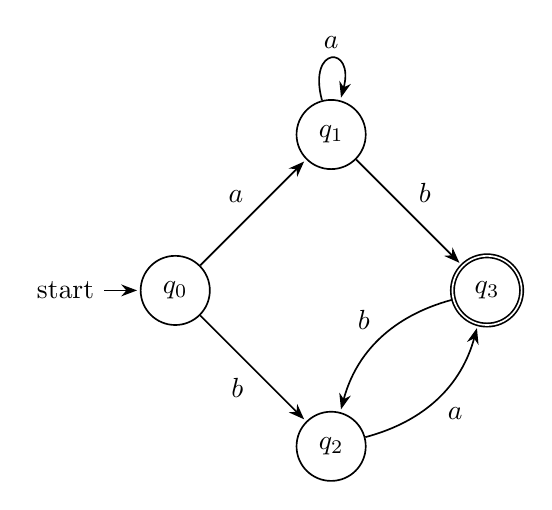
\begin{tikzpicture}[->, >=Stealth, shorten >=1pt, auto, node distance=2.8cm, on grid, semithick]
  \node[state, initial] (q0) {$q_0$};
  \node[state] (q1) [above right=of q0] {$q_1$};
  \node[state] (q2) [below right=of q0] {$q_2$};
  \node[state, accepting] (q3) [below right=of q1] {$q_3$};
  \path (q0) edge node {$a$} (q1)
             edge node [swap] {$b$} (q2)
        (q1) edge [loop above] node {$a$} ()
             edge node {$b$} (q3)
        (q2) edge [bend right] node [swap] {$a$} (q3)
        (q3) edge [bend right] node [swap] {$b$} (q2);
\end{tikzpicture}
\end{document}
